\documentclass[varwidth=true, border=2pt]{standalone}

\usepackage{pgfplots}
\usepackage{tikz}

\usetikzlibrary{calc,patterns,angles,quotes}

\begin{document}
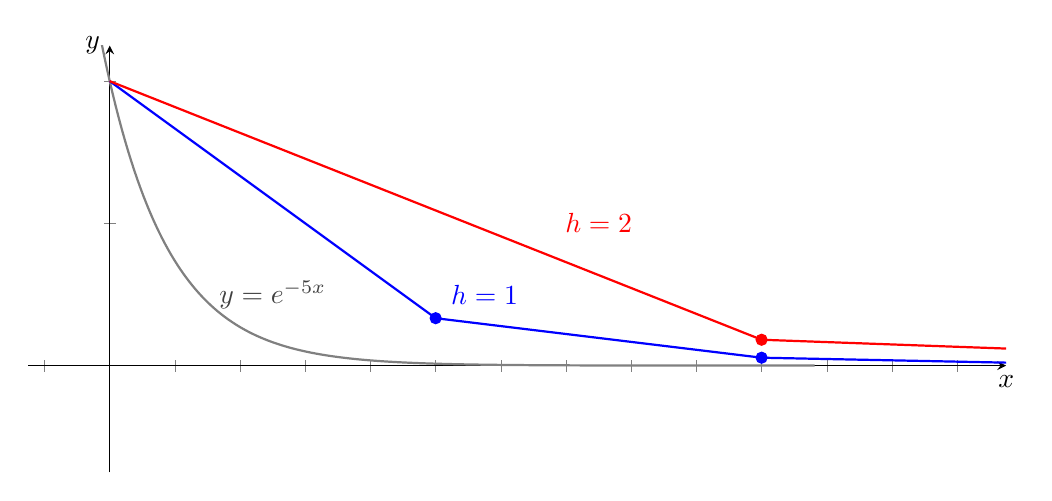
\begin{tikzpicture}
    \begin{axis}[
        legend pos=south east,
        axis x line=middle,
        axis y line=middle,
	every axis x label/.style={at={(current axis.right of origin)},anchor=north},
	every axis y label/.style={at={(current axis.above origin)},anchor=east},
	xticklabels=\empty,
	yticklabels=\empty
        grid = none ,
        width=14cm,
        height=7cm,
        grid style={dashed, gray!1},
        xmin=0,     % start the diagram at this x-coordinate
        xmax=2.5,    % end   the diagram at this x-coordinate
        ymin=-0.25,     % start the diagram at this y-coordinate
        ymax=1,   % end   the diagram at this y-coordinate
        xlabel=$x$,
        ylabel=$y$,
        enlargelimits=true,
        tension=0.08]


         \addplot[domain=-0.2:2.1625, gray,samples=250, thick] {exp(-5*x)};
         
         %  Step Size h = 1
         \node (X0) at (axis cs: 0,1) {};
         \node (A1) at (axis cs: 1,1/6) {};
         \node (A2) at (axis cs: 2, 1/36){};
         \node (A3) at (axis cs: 3, 1/216){};
         \draw [thick,blue] (X0.center) to (A1.center);
         \draw [thick,blue] (A1.center) to (A2.center);
         \draw [thick,blue] (A2.center) to (A3.center);
         \node (AL)[blue] at (axis cs: 1.15,0.25) {$h = 1$};
         
	%  Step Size h = 2
         \node (B1) at (axis cs: 2,1/11) {};
         \node (B2) at (axis cs: 4,1/121) {};
         \draw [thick,red] (X0.center) to (B1.center);
         \draw [thick,red] (B1.center) to (B2.center);
         \node (BL)[red] at (axis cs: 1.5,0.5) {$h = 2$};
         
         \node(E)[darkgray] at (axis cs: 0.5, 0.25){$y = e^{-5x}$};
         
         \addplot[red, only marks, mark=*] coordinates {(2,1/11)};
          \addplot[blue, only marks, mark=*] coordinates {(1,1/6)(2,1/36)};
         

    \end{axis}
\end{tikzpicture}
\end{document}